%!TEX root = ../template.tex
%%%%%%%%%%%%%%%%%%%%%%%%%%%%%%%%%%%%%%%%%%%%%%%%%%%%%%%%%%%%%%%%%%%%
%% chapter3_HardwareDesign.tex
%% NOVA thesis document file
%%
%% Chapter with the Hardware Design part
%%%%%%%%%%%%%%%%%%%%%%%%%%%%%%%%%%%%%%%%%%%%%%%%%%%%%%%%%%%%%%%%%%%%

\typeout{NT FILE chapter3_HardwareDesign.tex}

\chapter{Hardware Design}\label{cha:chapter3_HardwareDesign}

Meter aqui um pequena introdução do que e mostrado neste capitulo e descrição de seccoes

%SSSSSSSSSSSSSSSSSSSSSSSSSSSSSSSSSSSSSSSSSSSSSSSSSSSSSSSSSSSSSSSSSSSSSSSSSSSS
\section{Architecture and Component Selection}\label{sec:31_Architecture}

The system's desired specifications and requirements exposed throughout Section~\ref{sec:II_Specs} allow a redesign of its current architecture (Figure~\ref{fig:architecture_original}), which is presented in Figure~\ref{fig:architecture_new}.

% meter aqui o NOVO diagrama de blocos -- INACABADO;
\begin{figure}[h]
	\centering
	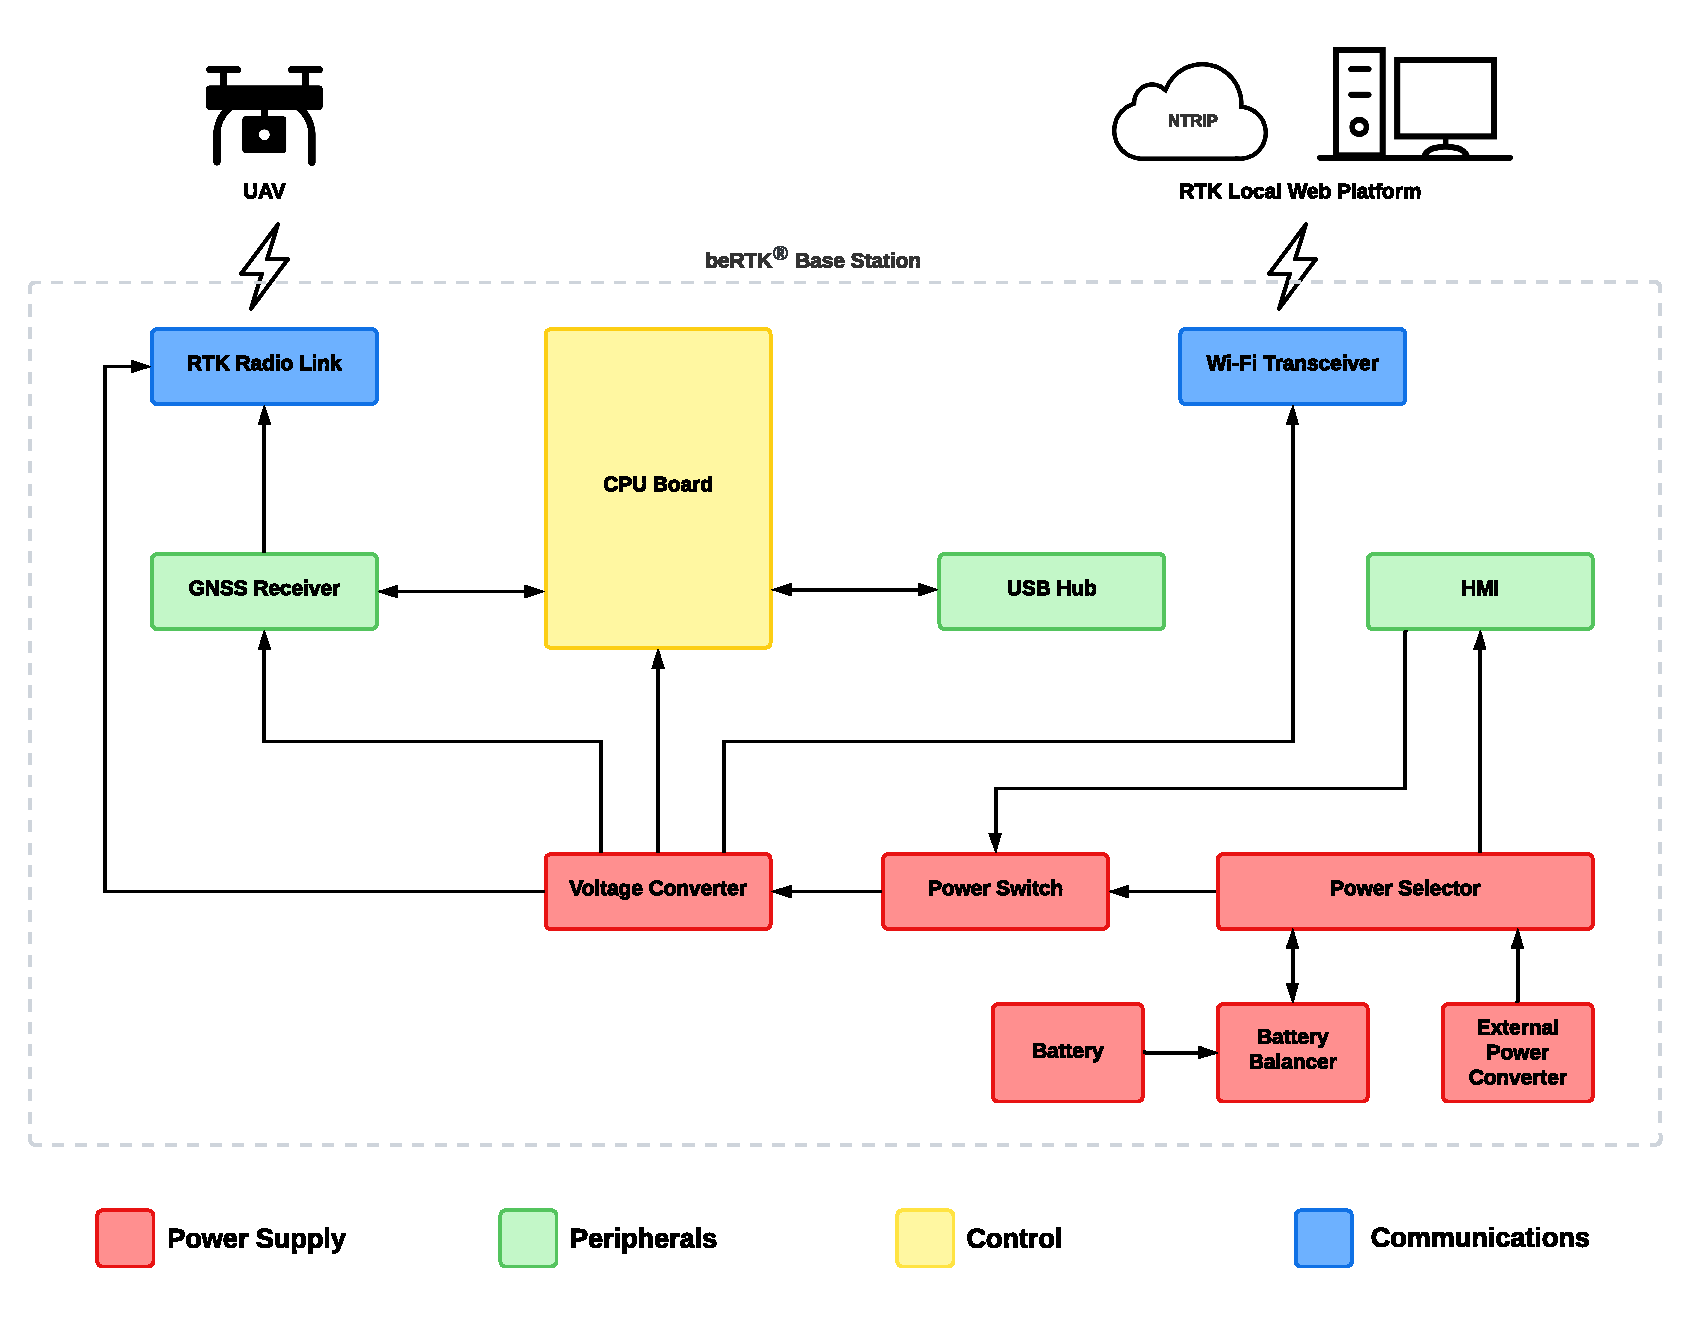
\includegraphics[width=1.0\textwidth]{Chapters/Figures/new_architecture_2.pdf}
	\caption{beRTK\textsuperscript{\textregistered} Base Station's redesigned block diagram.}
	\label{fig:architecture_new}
\end{figure}

%VER SE ESTA ORDEM DE SUBCAPITULOS É BOA O SUFICIENTE, ou se tenho de a alterar

%sSsSsSsSsSsSsSsSsSsSsSsSsSsSsSsSsSsSsSsSsSsSsSsSsSsSsSsSsSsSsSsSsSsSsSsSsSsS
\subsection{Control}\label{sec:311_Control}

Starting from the control subgroup, the only component to be selected was a single-board computer able to replace the previously used Raspberry Pi 4 Model B; this means the chosen device would have to be able to carry out a pre-determined set of instructions crucial for the operation of the base station. Such requirement is presented in Section~\ref{sec:II_FCT_requirements} -- requirement \textbf{RTKBS.MAIN.FCT.030}, which proposes the use of a single-board computer (SBC).
The set of instructions performed by the original beRTK\textsuperscript{\textregistered} base station is carried out by a Raspberry Pi 4 Model B computer (described in Section~\ref{sec:II_architecture_Control}), therefore, an element with a comparable computational power as this computer would be ideal. The Raspberry Pi Foundation offers a variety of solutions for many project ideas\footnote[7]{The Raspberry Pi Foundation's hardware offers are available at \url{https://www.raspberrypi.com/products/}.}, and since the operations intended for the beRTK\textsuperscript{\textregistered} base station are so well performed by the Raspberry Pi 4 Model B, it would be worth looking through the array of Raspberry Pi products in order to find a good solution. Research leads to the Raspberry Pi Compute Module 4.
This compact module not only has a small form factor when compared with the Raspberry Pi 4 Model B, but it also bears its computational power thanks to the same processor (a Broadcom BCM2711 quad-core Cortex-A72 (ARM v8) 64-bit SoC @ 1.5GHz), which makes it a great option for the system's control unit~\cite{CM4}.

%meter imagem CM4:
\begin{figure}[h]
	\centering
	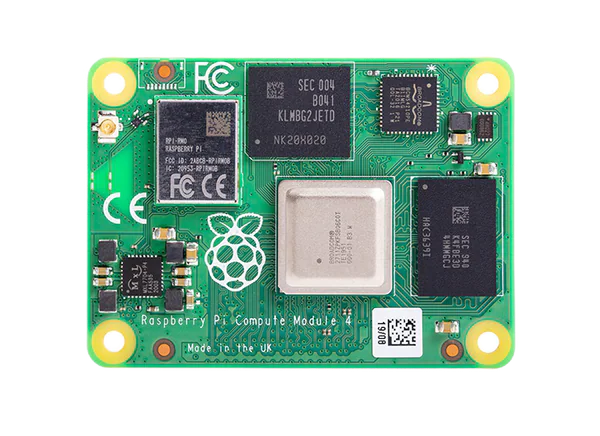
\includegraphics[width=0.5\textwidth]{Chapters/Figures/CM4.png}
	\caption{The Raspberry Pi Compute Module 4 (CM4)~\cite{CM4}.}
	\label{fig:CM4}
\end{figure}

One can choose from thirty-two CM4 variants which differ from each other on RAM and eMMC flash, as well as with or without wireless capabilities.

%sSsSsSsSsSsSsSsSsSsSsSsSsSsSsSsSsSsSsSsSsSsSsSsSsSsSsSsSsSsSsSsSsSsSsSsSsSsS
\subsection{Peripherals and Communications}\label{sec:312_Peripherals_Communications}

Since this module is intended to be an embedded solution without any of the external ports present in the Raspberry Pi 4 Model B, the relevant ones must be included in the proposed solution, which in this case are USB and HDMI. The CM4 provides all the necessary pins for the implementation of two HDMI connectors on its carrier board (in this case the base station); however, when it comes to using its USB interface, the user must add a USB hub, since only two USB data pins are provided, along with a USB On-The-Go (OTG) pin. The latter is used in order to define the CM4 as either a host or a slave~\cite{CM4}.

%meter imagem do HUB usb: LAN9514

In order to enable such data transfers, the base station would need a component designed to allow the setup of both upstream and downstream USB ports. The Raspberry Pi 3 Model B uses a chip known as LAN9514, which is a four-port USB hub with ethernet functionality. Since this chip has the needed characteristics for the setup of the CM4's USB interface, it was chosen as the main module concerning USB data transfer.

The datasheet for LAN9514 details the chip as a 10/100 ethernet controller, as well as a USB 2.0 hub with four downstream ports and one upstream port, and targets it for desktop computers and embedded systems, among other uses~\cite{LAN9514}. The LAN9514 also fits the Peripherals subgroup, along with the ZED-F9P GNSS receiver and the HMI, the latter of which bridges the user-device gap via a simple on/off button, LED indicators for both battery status and power source indication and a single connector intended for an external power source, satisfying requirement \textbf{RTKBS.MAIN.PWS.050}, as well as all the requirements defined in Section~\ref{sec:II_HMI_requirements}.

It is also worth mentioning that, referring to requirements \textbf{RTKBS.MAIN.FCT.020} and \textbf{RTKBS.MAIN.FCT.040}, which correspond to the GNSS receiver (ZED-F9P) and the Wi-Fi transceiver (Digi XBee\textsuperscript{\textregistered} 3), respectively, there were no changes in such elements for the new beRTK\textsuperscript{\textregistered}'s proposed solution.

%sSsSsSsSsSsSsSsSsSsSsSsSsSsSsSsSsSsSsSsSsSsSsSsSsSsSsSsSsSsSsSsSsSsSsSsSsSsS
\subsection{Power Supply}\label{sec:313_PowerSupply}

The secondary power arrangement in the original beRTK\textsuperscript{\textregistered} design features two external batteries that would feed the entire system once the mains power supply was disconnected. This form of supply poses considerable disadvantages when it comes to a continuous operation, due to the impractical need of removing the batteries in order to charge them. In the system's power supply subgroup, this was the main improvement to be made following the requirements defined in Section~\ref{sec:II_PWS_requirements}. For that, the base station's enclosure sould count on an internal battery (requirement \textbf{RTKBS.MAIN.PWS.020}) that must not be removed (such battery could be comprised of either a single or multi-cell arrangement) on which the system could rely once the external power supply was disconnected. This idea would help meet requirement \textbf{RTKBS.MAIN.MEC.030}, proposing however a new issue, namely, the charging of the internal battery arrangement.
%meter hyperLINK PARA CADA REQUIREMENT

The original beRTK\textsuperscript{\textregistered}'s design also features a prioritized PowerPath\textsuperscript{\texttrademark} controller, as mentioned in Section~\ref{sec:II_architecture_PowerSupply}.
As per Analog Devices, a PowerPath\textsuperscript{\texttrademark} controller is a device able to control the flow of power through a system, while also selecting its power source.
With this in mind, a wise starting point for the research of a power selector able to provide a smooth transistion between an external and internal supply would be from Analog Devices' power management ICs; specifically, from the battery charger IC catalogue. The most well-suited IC found was LTC4012, which is a high efficiency, multi-chemistry battery charger with PowerPath\textsuperscript{\texttrademark} control. This battery charger offers an adjustable output voltage, as well as the option to program a charging current for the circuit's internal battery~\cite{LTC4012}.

Taking into account requirement \textbf{RTKBS.MAIN.PWS.010} -- which regards the system's input \gls{DC} voltage (from +7 VDC to +22 VDC) -- and the battery charger's input voltage range (from +6 VDC to +28 VDC), the intermediary value of +15 VDC was chosen as the main DC input voltage for the system. This value was taken as reference for the calculations made througout the circuit design phase.
%falar de como a PWM permite um switching smooth entre external power para as baterias

%depois falar do sistema operativo

%depois falar da local web platform
	% da configuraçao dos parametros da base atraves dessa plataforma
	% dos log que podem ser obtidos atraves da operaçao da base


%SSSSSSSSSSSSSSSSSSSSSSSSSSSSSSSSSSSSSSSSSSSSSSSSSSSSSSSSSSSSSSSSSSSSSSSSSSSS
\section{Circuit Design}\label{sec:32_Circuit}

%meter uma pequena introduçao a dizer que usei o kicad e que segui uma metodologia qualquer

%sSsSsSsSsSsSsSsSsSsSsSsSsSsSsSsSsSsSsSsSsSsSsSsSsSsSsSsSsSsSsSsSsSsSsSsSsSsS
\subsection{Power Supply}\label{sec:321_POWERSUPPLY}
	%mini introdução

%s--Ss--Ss--Ss--Ss--Ss--Ss--Ss--Ss--Ss--Ss--Ss--Ss--Ss--Ss--Ss--Ss--Ss--Ss--S
\subsubsection{Power Selector}\label{sec:3211_LTC4012}

\paragraph{Programming the Charge Current}	When it comes to powering the system through different sources, maintaining its continuous operation when switching between said sources is crucial. The LTC4012 battery charger is able to accomplish just that: this buck converter relies on a synchronous quasi-constant frequency \gls{PWM} control architecture and is able to provide a connected battery pack with a charge current programmed through external resistors. Since it does not have a built-in termination, it is capable of charging a broad range of batteries at a maximized rate and effieciency -- for a given established power level --, due to an existing \gls{AC} adapter current limiting feature, possible to program and monitor via an external sense resistor. For this project, an arrangement of two rechargeable Lithium-ion (Li-ion) cells in series (also known as a ``2S Li-ion battery'') was chosen as the backup battery pack for the system, with each of the cells offering $3,350$mAh worth of capacity. It must be noted that a set of two cells in series does not alter the pack's total capacity, therefore this same specification will remain the same for the backup battery -- $3,350$mAh.

With this in mind, studying the battery cell's datasheet reveals that each battery -- and therefore, the 2S arrangement -- is capable of being charged with a recommended standard charge of $1,700$mA~\cite{INR18650-35E}.
Figure~\ref{fig:battery2S} and Table~\ref{tab:battery2S} show a close-up representation and typical characteristics of a single cell, respectively.

%imagem e Table da bateria aqui:

\begin{figure}[h]
	\centering
	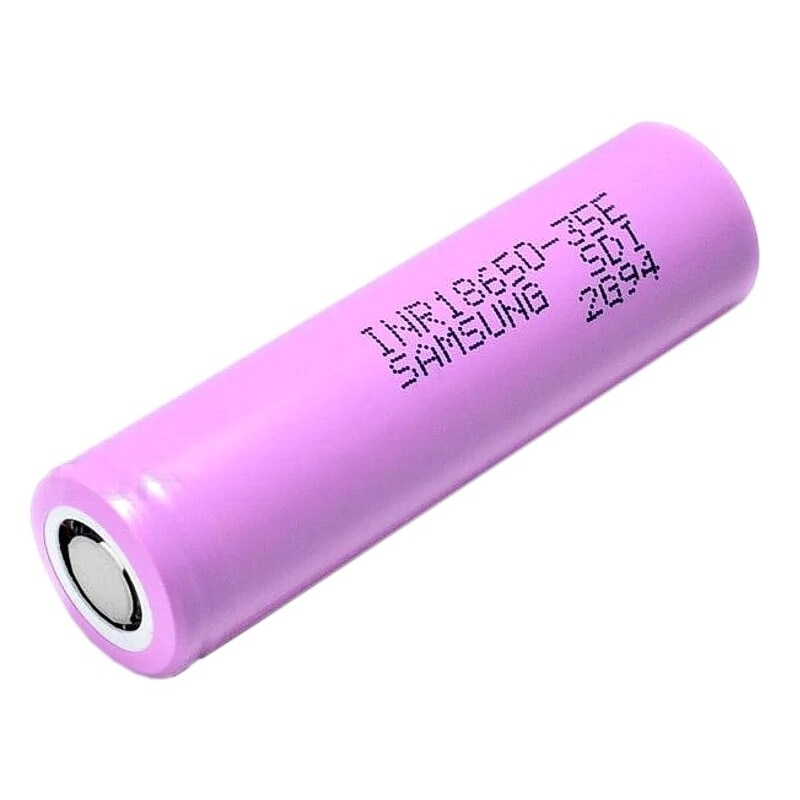
\includegraphics[width=0.4\textwidth]{Chapters/Figures/chapter3/bateria-li-ion-mr-18650-3-6v-3500mah-samsung-inr18650-35e.jpg}
	\caption{Visual representation of the type of battery cell used.}
	\label{fig:battery2S}
\end{figure}

\begingroup
\begin{table}[h]
	\caption{Typical characteristics of the type of battery cell used~\cite{INR18650-35E}.}
	\label{tab:battery2S}
	\centering%@{}l@{}@{}c@{}@{}c@{}@{}c@{}@{}c@{}
    % \setlength{\tabcolsep}{10pt} % Default value: 6pt
    % \renewcommand{\arraystretch}{1.5} % Default value: 1
	\begin{tabular}{lc}
        \toprule
        \textbf{Specification} & \textbf{Value} \\
        \midrule
        Manufacturer & Samsung SDI \\
        \midrule
        Model & INR18650-35E \\
        \midrule
		Size & 18650 \\
		\midrule
		Chemistry & Li-ion \\
		\midrule
		Capacity & 3,350mAh \\
        \midrule
		Charging Cycle Termination Voltage & 4.20V $\pm$ 0.05V \\
		\midrule
		Nominal Voltage & 3.60V \\
        \midrule
		Charging Current (standard charge) & 1,700mA\\
		\midrule
		Charging Current (for life cycle) & 1,020mA\\
		\midrule
		Maximum Charge Current (not for life cycle) & 2,000mA \\
		\midrule
		Maximum Discharge Current (continuous discharge) & 8,000mA \\
		\midrule
		Maximum Discharge Current (not for continuous discharge) & 13,000mA \\
		\midrule
		Discharge Cut-off Voltage & 2.65V \\
        \bottomrule
    \end{tabular}
\end{table}
\endgroup

Table~\ref{tab:battery2S} specifies that each battery provides a charging cycle termination voltage of approximately 4.20V, which bespeaks that the 2S arrangement adds up to a total of (approximately) 8.40V of backup energy.

It is possible to calculate an estimate of the system's battery life using expression~(\ref{eq:battery_life}):

\begin{equation}\label{eq:battery_life}
    \textrm{Battery Life} = \frac{\textrm{Battery Capacity (mAh)}}{\textrm{Load Current (mAh)}} = \frac{3350}{1000} = 3.35 \textrm{ hours}\,\medskip
\end{equation}

\noindent Assuming a total system load current of approximately $1,000$mA results in an expected total battery life of roughly 3.35 hours. That estimate corresponds to, roughly, three-and-a-half hours of work time. Of course one must account for the unideal characteristics of the real world acting upon the system, but nevertheless, this expression serves as a guideline/reminder for an expected power consumption of the base station's circuit. 

The LTC4012 datasheet provides a helpful typical application circuit, as well as the device's application information. These two key sections of the document allowed an adapted development of the power selection circuit of the new beRTK\textsuperscript{\textregistered}, presented by the schematic diagram in Figure~\ref{fig:LTC4012_circuit}. Following the application information of the product started by programming the charge current which would be used to replenish the energy back to the battery pack. For that, formula~\ref{eq:i_chrg} is provided:

\begin{equation}\label{eq:i_chrg}
    I_{CHRG}=\frac{R_{IN}}{R_{SENSE}} \cdot \left(\frac{1.2085\textrm{V}}{R_{PROG}}-11.67\mu\textrm{A}\right)\,\medskip
\end{equation}

\noindent The $I_{CHRG}$ charge current is programmed by selecting the $R_{IN}$, $R_{SENSE}$ and $R_{PROG}$ resistors. $R_{SENSE}$ (sense resistor) can be selected through expression~(\ref{eq:r_sense}),

\begin{equation}\label{eq:r_sense}
    R_{SENSE}=\frac{100 \textrm{mV}}{I_{MAX}}\,,\medskip
\end{equation}
where $I_{MAX}$ corresponds to the maximum $I_{CHRG}$ charge current desired for the charging process. As per Table~\ref{tab:battery2S}, the battery pack allows a maximum charge current of $2,000$mA, but this value does not account for the maintenance of each cell's health. For that, a standard charging current of $1,700$mA is mentioned in the datasheet; in C-rate units, this charging current rate corresponds to 0.5C, since the explicit 1C rate for this type of cell is equal to $3,400$mA\footnote[8]{In the C-rate standard, 1C corresponds to a charging from 0 to 100\% in the span of one hour. The higher the C-rate coefficient, the faster the charge, and vice-versa. For example, a rate of 2C corresponds to thirty minutes of charge time and 0.5C to two hours.}~\cite{C-rate}.
However, it is also pointed out that, in order to maintain the batteries' health as pristine as possible (thus prolonging their life cycle), a charge current of $1,020$mA -- i.e. maintaining the cell's C-rate of 0.3C -- would have to be employed. Choosing a maximum charge current of $I_{MAX}=1,020$mA results in an $R_{SENSE}$ value of 0.098$\Omega$ (98m$\Omega$), according to~(\ref{eq:r_sense}) (represented in the schematic of Figure~\ref{fig:LTC4012_circuit} by R12). Therefore, the value of $I_{MAX}=1,020$mA is hereby defined as the 1C rate of the new beRTK\textsuperscript{\textregistered}'s battery pack. It should also be noted that the target sense voltage of 100mV can differ in order to accomodate standard $R_{SENSE}$ values available on the market, however lower values are likely to cause inaccuracies when it comes to current regulation.

% meter aqui circuito do LTC4012:
\begin{figure}[h]
	\centering
	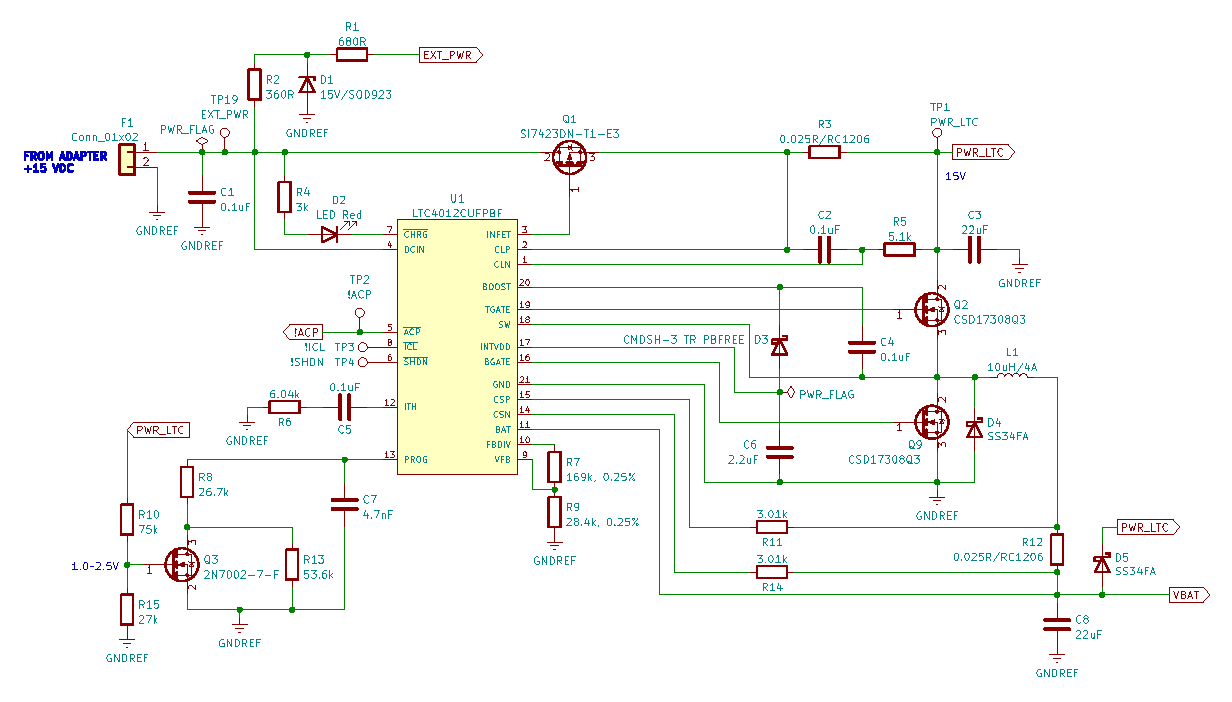
\includegraphics[width=1.0\textwidth]{Chapters/Figures/chapter3/Power_Supply_and_Selection.pdf}
	\caption{beRTK\textsuperscript{\textregistered} Base Station's Power Supply and Selection schematic diagram.}
	\label{fig:LTC4012_circuit}
\end{figure}

It is established in the documentation that the LTC4012 provides the best performance with two equal 3.01k$\Omega$ $R_{IN}$ input resistors\footnote[9]{Other input resistor values can also be used in order to adjust to different standard sense resistor value that could be chosen~\cite{LTC4012}.} (represented in Figure~\ref{fig:LTC4012_circuit} by R11 and R14). This input resistor value is used for the calculation of the minimum resistance required between the PROG pin and \gls{GND}, given by (\ref{eq:r_prog}).

\begin{equation}\label{eq:r_prog}
    R_{PROG (MIN)}=\frac{1.2085 \textrm{V} \cdot R_{IN}}{0.1 \textrm{V} + 11.67 \mu \textrm{A} \cdot R_{IN}} \approx 26.9 \textrm{k}\Omega \,\medskip
\end{equation}

\noindent Expression (\ref{eq:r_prog}) results in a minimum $R_{PROG}$ value of approximately 26.9k$\Omega$, and connecting a resistor of this value between the PROG pin and GND is enough to control the maximum charge current of $I_{MAX}$ (i.e. 1C).

% \noindent Expression (\ref{eq:r_prog}) results in a minimum $R_{PROG}$ value of approximately 26.9k$\Omega$, and connecting a resistor of this value between the PROG pin and GND would be sufficient if the only charge current rate defined was $I_{MAX}$ (i.e. 1C).
% However, when batteries discharge to a voltage level below their minimum specified recommendation (in the case of the cells used, 2.5V), they suffer internal damage, which results -- in the long run -- in a loss of battery life.
% Therefore, when the aforesaid situation occurs, the charging process should be done with a low initial charge current. Such practice also ensures an overall safe charging of the baterries, regardless of whether or not a heavy discharge has taken palce.
% The LTC4012 charger allows a specific charging control process for the battery pack by altering the resistance between the PROG pin and GND, designated as a ``two-level'' charge. This charging process is achieved via the switching of a control transistor (Q3 in Figure~\ref{fig:LTC4012_circuit}) which, when turned off, cuts down the charge current to $\frac{I_{MAX}}{10}$ (i.e. C/10), only allowing the full $I_{MAX}$ current for a ``bulk charge'' when turned on. In the schematic of Figure~\ref{fig:LTC4012_circuit}, the two-level approach is implemented through transistor Q3, resistors R8 and R13 and capacitor C7. Connecting the gate of Q3 to the battery supply rail ($\mathrm{V_{BAT}}$ net in Figure~\ref{fig:LTC4012_circuit}) serves the purpose of allowing transistor Q3 to exit or enter its active zone, in order to subsequently grant both levels of charge current available with the implemented method. When the battery pack's voltage dips to a value equal to or below 2.5V -- i.e. when it reaches a heavy discharge status --, Q3 is switched on, increasing (MENTIRA! ELE DIMINUI A RESISTENCIA...) the resistance between PROG and GND. For that, the recommended transistor to use (from the LTC4012 datasheet) is the 2N7002 N-channel \gls{FET}~\cite{2N7002}. This FET holds a gate threshold voltage between 1.0V and 2.5V.
%DESCARTEI O 2-LEVEL CHARGE.

With the calculated values for resistors $R_{IN}$, $R_{SENSE}$ and $R_{PROG}$ it is then possible to obtain a value of $I_{CHRG} = 1,020$mA for the programmed charge current, through expression~(\ref{eq:i_chrg}).

\paragraph{Programming the LTC4012 Output Voltage}	An external resistor divider circuit can be assembled in order to set an output voltage for the charger. This circuit is composed by resistors R7 and R9 from Figure~\ref{fig:LTC4012_circuit}, whose approximate values are suggested in the LTC4012 datasheet. For a $V_{BAT}$ voltage of 8.40V, these values are 169k$\Omega$ and 28.4k$\Omega$, respectively, and can be confirmed through equations (\ref{eq:v_bat}) and (\ref{eq:r7_r9}):

\begin{equation}\label{eq:v_bat}
    V_{BAT}=\frac{1.2085\textrm{V} \cdot \left(R7 + R9\right)}{R9}\,\medskip
\end{equation}

\begin{equation}\label{eq:r7_r9}
    R7=R9 \cdot \left(\frac{V_{BAT}}{1.2085\textrm{V}} - 1\right)\,\medskip
\end{equation}

If the selected value of R9 is less than 50k$\Omega$ and the joint value of R7 and R9 surpasses (or at least equals) 200k$\Omega$, then the lowest possible error at the $V_{FB}$ sense input is acheived\footnote[10]{The use of resistors with a tolerance level of 0.25\% is advised to achieve the desired level of accuracy~\cite{LTC4012}.}. It should be noted that the influence of this battery voltage feedback input is present in equations (\ref{eq:v_bat}) and (\ref{eq:r7_r9}), as well as in equations (\ref{eq:i_chrg}) and (\ref{eq:r_prog}), in the form of the nominal 1.2085 pin voltage.

\paragraph{Programming the Input Current Limit}	The previous version of the beRTK\textsuperscript{\textregistered} base station presented a power consumption of approximately 3 to 3.5Wh, and one of the requirements of this project is to cut the power consumption down to a maximum of 400mA at +5VDC -- as stated in requirement \textbf{RTKBS.MAIN.PWS.040}. Therefore, a 1.00A external adapter current rating can safely be considered, however, it is best to consider the double of that value, to safely consider high peak currents and discharge problems that may arise.
The LTC4012 datasheet provides a table with common values for a sense resistor dedicated to the programming of the input current limiting -- R3 in Figure~\ref{fig:LTC4012_circuit}. For this case, considering an adapter rating of 2.00A, R3's estimated value would be equal to 0.050$\Omega$ (50m$\Omega$). The value of this sense resistor can also be determined through expression (\ref{eq:r_cl}),

\begin{equation}\label{eq:r_cl}
    R3=\frac{100\textrm{mV}}{I_{LIM}}\,,\medskip
\end{equation}
where $I_{LIM}$ corresponds to the desired maximum current able to be drawn from the external adapter input -- in this case, that value was chosen to be 2.00A. The LTC4012 also provides a pin named $\overline{\mbox{ICL}}$, an active-low indicator output that immediately pulls to GND upon the detection of a reduction of the charge current (due to the aforementioned AC adapter input current limiting).

The switching noise generated by the PWM control architecture and different system components can be canceled out by a low-pass filter consisting of resistor R5 (5.1k$\Omega$) and capacitor C2 (0.1$\mu$F) -- also present in Figure~\ref{fig:LTC4012_circuit} --, between the charger's CLP and CLN pins.

% \paragraph{The $\mathbf{\frac{C}{10}}$ $\mathbf{\overline{CHRG}}$ Indicator}	As stated before, when the N-channel FET Q3 (2N7002) is turned off, the maximum charge current allowed is $\frac{I_{MAX}}{10}$, which helps preserve the battery's health. This FET allows the setting of two different values for the total external resistance between the PROG pin and GND of the LTC4012 -- composed by resistors R8 and R13 of Figure~\ref{fig:LTC4012_circuit} --, which enables the programming of the battery pack's charge current. Along with this resistance, the R12 current sense resistor and PWM input resistors (R7 and R9) also play an important role on setting said charge current, since information about the current battery level is necessary so that the device can detect if a heavy discharge has taken place (i.e. the discharge cut-off voltage of 2.65V has been reached), in order to only allow the $\frac{I_{MAX}}{10}$ charge current. The LTC4012 provides a dedicated pin 

\paragraph{Input and Output Capacitors}	Within a single system, different circuits can share the same nets, the most common of which are usually power and ground. Power supply signals often carry residual noise known as ripple voltage, which, when present, can be harmful towards components such as integrated circuits. A way to attenuate such noise is through the use of capacitors known as decoupling (or bypass) capacitors. These components help guarantee the continuous power supply to the differnet sub-circuits when changes in the system load occur -- which result in voltage drops caused by shifting currents -- while also doing their best to cancel out surges of high-frequency noise that may spread to other parts of the system, reducing the generated \gls{EMI}. 

The LTC4012's +15 VDC power input (pin DCIN) requires a supply bypassing capacitor to help reduce the \gls{ringing} caused by AC adapter \gls{hot-plugging}. A $0.1 \mu$F aluminium electrolytic capacitor is recommended (due to the relatively high \gls{ESR}). If not available, a $20 \mu$F ceramic capacitor (considered a high capacity for this type of capacitor) can be used for this power input, as well as the power output. The latter capacitor (C8 in Figure~\ref{fig:LTC4012_circuit}; placed across the battery and the GND terminal) is intended for PWM output ripple current absorbtion and its value can be calculated through formula (\ref{eq:i_rms}),

\begin{equation}\label{eq:i_rms}
    I_{RMS}=\frac{0.29 \cdot V_{BAT} \cdot \left(1-\frac{V_{BAT}}{V_{CLP}}\right)}{\textrm{L1} \cdot f_{PWM}}\,,\medskip
\end{equation}
where		% PAREI AQUI

An input capacitor between the drain of the top FET (Q2 in Figure~\ref{fig:LTC4012_circuit}) and GND should also be placed, concerning the attenuation of all the input PWM current which may come through.

%if a $0.1 \mu$F aluminium electrolytic capacitor is not availabe, use a 20uF ceramic capacitor

% REFERÊNCIA needed!!!!!!!!!!!!!!!!!!!!
%s--Ss--Ss--Ss--Ss--Ss--Ss--Ss--Ss--Ss--Ss--Ss--Ss--Ss--Ss--Ss--Ss--Ss--Ss--S
\subsubsection{Battery Balancer}\label{sec:3212_BQ29209}

% meter aqui circuito do BQ29209
\begin{figure}[h]
	\centering
	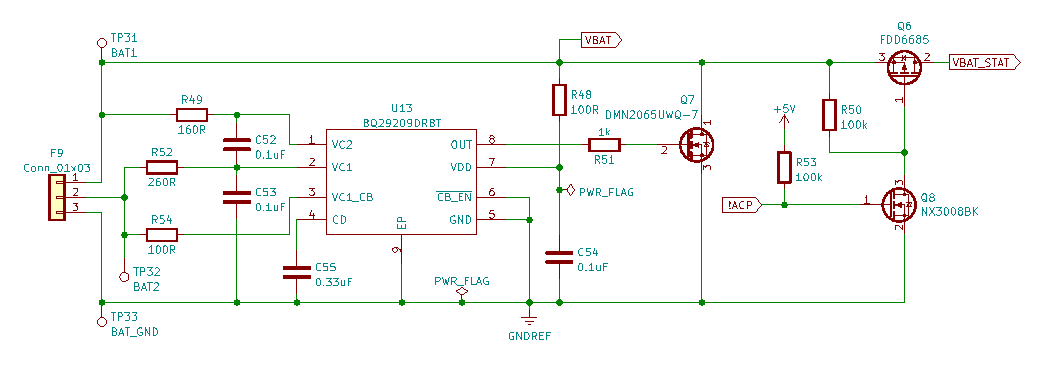
\includegraphics[width=1.0\textwidth]{Chapters/Figures/chapter3/Battery_Balancer.pdf}
	\caption{beRTK\textsuperscript{\textregistered} Base Station's Battery Balancer schematic diagram.}
	\label{fig:BQ29209_circuit}
\end{figure}

% REFERÊNCIA needed!!!!!!!!!!!!!!!!!!!!
%s--Ss--Ss--Ss--Ss--Ss--Ss--Ss--Ss--Ss--Ss--Ss--Ss--Ss--Ss--Ss--Ss--Ss--Ss--S
\subsubsection{Voltage Converter}\label{sec:3213_AP64501}

% meter aqui circuito do AP64501
\begin{figure}[h]
	\centering
	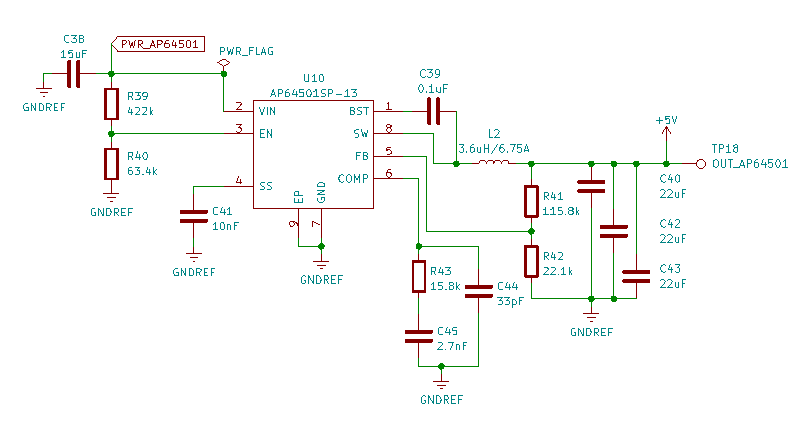
\includegraphics[width=1.0\textwidth]{Chapters/Figures/chapter3/Voltage_Converter.pdf}
	\caption{beRTK\textsuperscript{\textregistered} Base Station's Voltage Converter schematic diagram.}
	\label{fig:AP64501_circuit}
\end{figure}

% REFERÊNCIA needed!!!!!!!!!!!!!!!!!!!!
%s--Ss--Ss--Ss--Ss--Ss--Ss--Ss--Ss--Ss--Ss--Ss--Ss--Ss--Ss--Ss--Ss--Ss--Ss--S
\subsubsection{Power Switch}\label{sec:3214_SWITCH}

% meter aqui circuito do Power SWITCH
\begin{figure}[h]
	\centering
	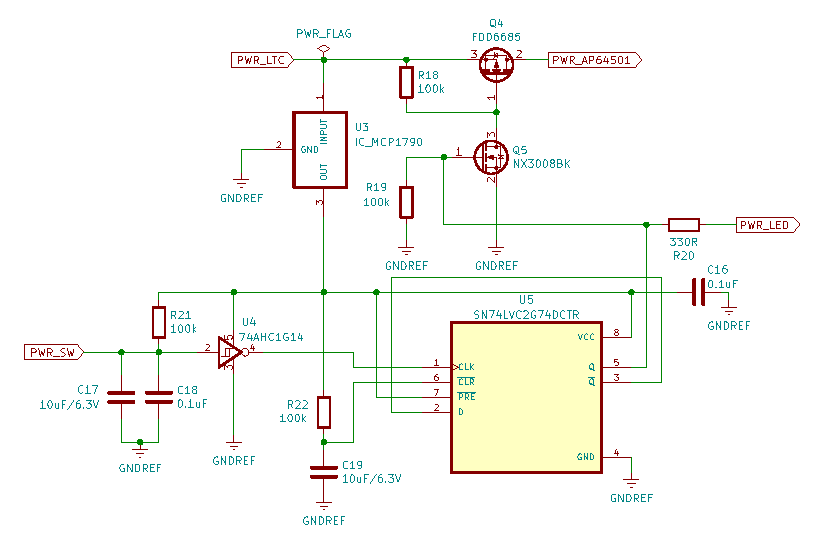
\includegraphics[width=1.0\textwidth]{Chapters/Figures/chapter3/Power_Switch.pdf}
	\caption{beRTK\textsuperscript{\textregistered} Base Station's Power Switch schematic diagram.}
	\label{fig:SWITCH_circuit}
\end{figure}

% REFERÊNCIA needed!!!!!!!!!!!!!!!!!!!!
%sSsSsSsSsSsSsSsSsSsSsSsSsSsSsSsSsSsSsSsSsSsSsSsSsSsSsSsSsSsSsSsSsSsSsSsSsSsS
\subsection{Control}\label{sec:322_CONTROL}
	%mini introdução

%s--Ss--Ss--Ss--Ss--Ss--Ss--Ss--Ss--Ss--Ss--Ss--Ss--Ss--Ss--Ss--Ss--Ss--Ss--S
\subsubsection{CPU Board -- GPIO}\label{sec:3221_CM4_GPIO}

% meter aqui circuito do CM4_GPIO
\begin{figure}[h]
	\centering
	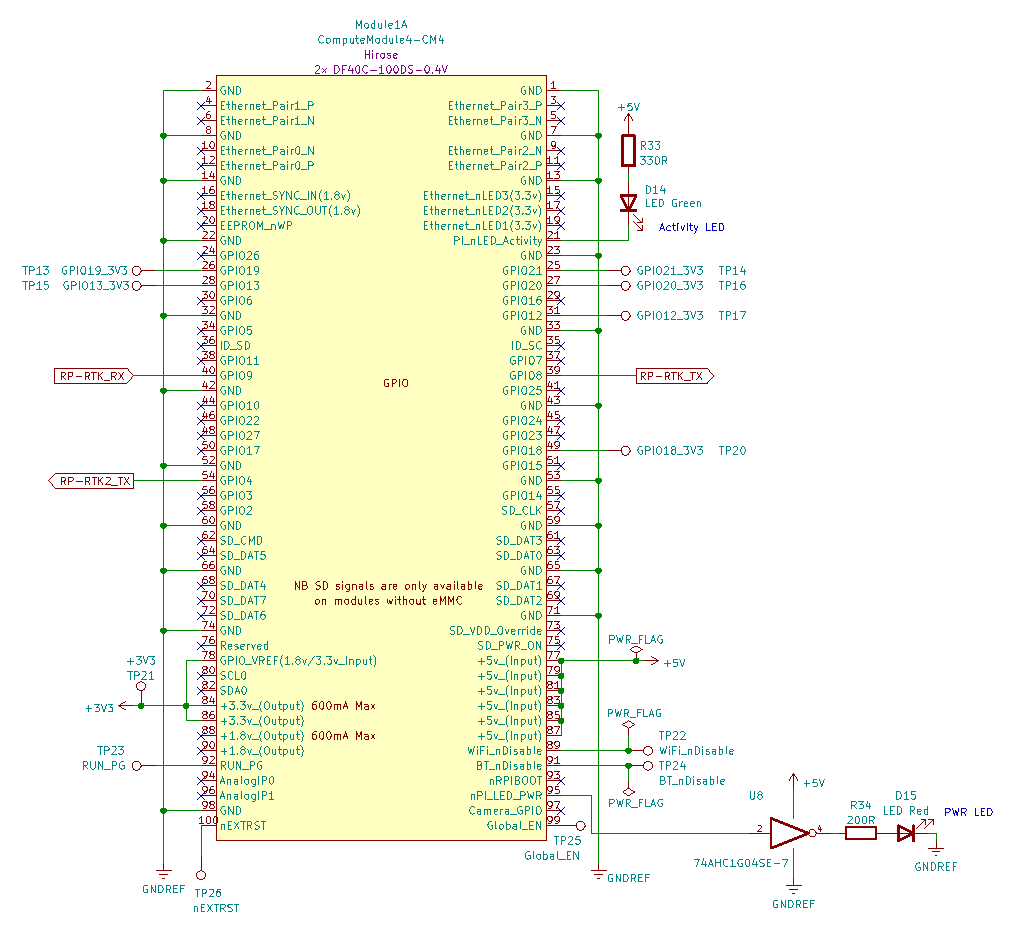
\includegraphics[width=1.0\textwidth]{Chapters/Figures/chapter3/CM4_GPIO.pdf}
	\caption{beRTK\textsuperscript{\textregistered} Base Station's CM4's GPIO schematic diagram.}
	\label{fig:CM4_GPIO_circuit}
\end{figure}

% REFERÊNCIA needed!!!!!!!!!!!!!!!!!!!!
%s--Ss--Ss--Ss--Ss--Ss--Ss--Ss--Ss--Ss--Ss--Ss--Ss--Ss--Ss--Ss--Ss--Ss--Ss--S
\subsubsection{CPU Board -- High-Speed}\label{sec:3222_CM4_HSpeed}

% meter aqui circuito do CM4_HighSpeed
\begin{figure}[h]
	\centering
	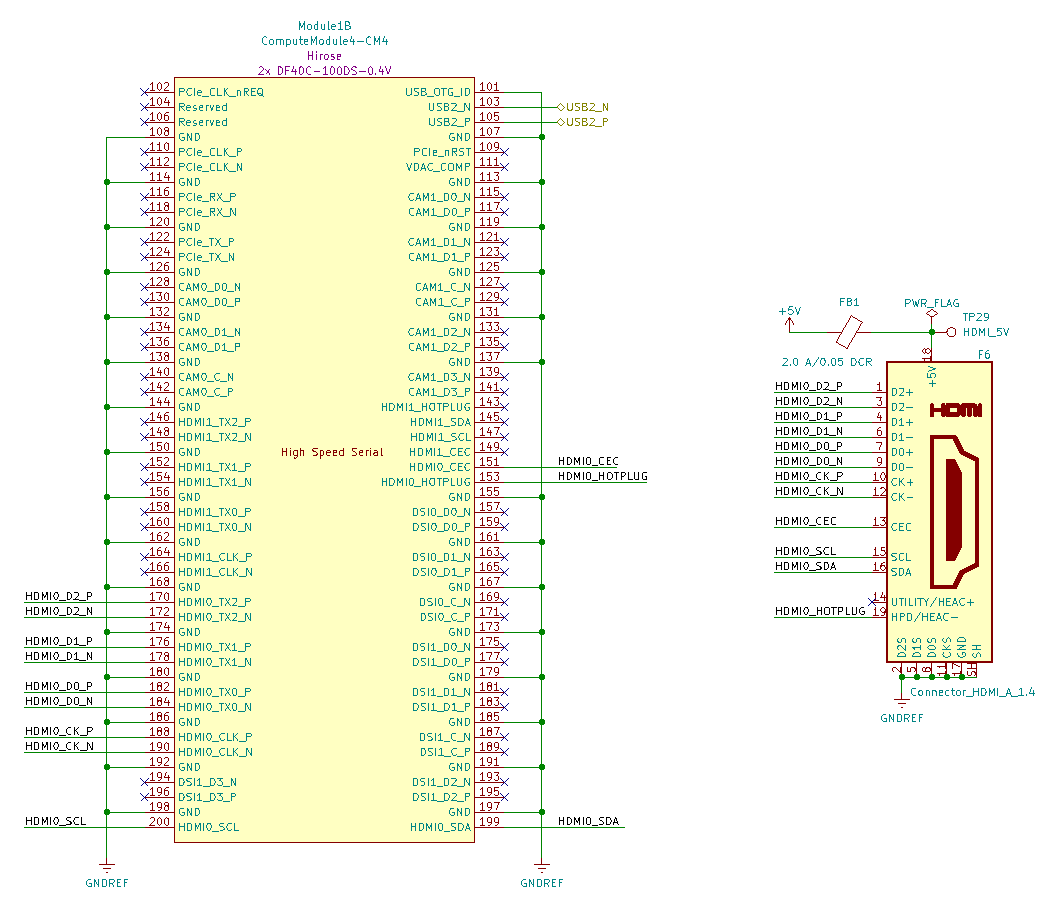
\includegraphics[width=1.0\textwidth]{Chapters/Figures/chapter3/CM4_HighSpeed.pdf}
	\caption{beRTK\textsuperscript{\textregistered} Base Station's CM4's High Speed schematic diagram.}
	\label{fig:CM4_HighSpeed_circuit}
\end{figure}

% REFERÊNCIA needed!!!!!!!!!!!!!!!!!!!!
%sSsSsSsSsSsSsSsSsSsSsSsSsSsSsSsSsSsSsSsSsSsSsSsSsSsSsSsSsSsSsSsSsSsSsSsSsSsS
\subsection{Peripherals and Communications}\label{sec:323_PERIPHERALS_COMMS}
	%mini introdução

%s--Ss--Ss--Ss--Ss--Ss--Ss--Ss--Ss--Ss--Ss--Ss--Ss--Ss--Ss--Ss--Ss--Ss--Ss--S
\subsubsection{Human-Machine Interface (HMI)}\label{sec:3231_BACKPANEL}

% meter aqui circuito do BACKPANEL
\begin{figure}[h]
	\centering
	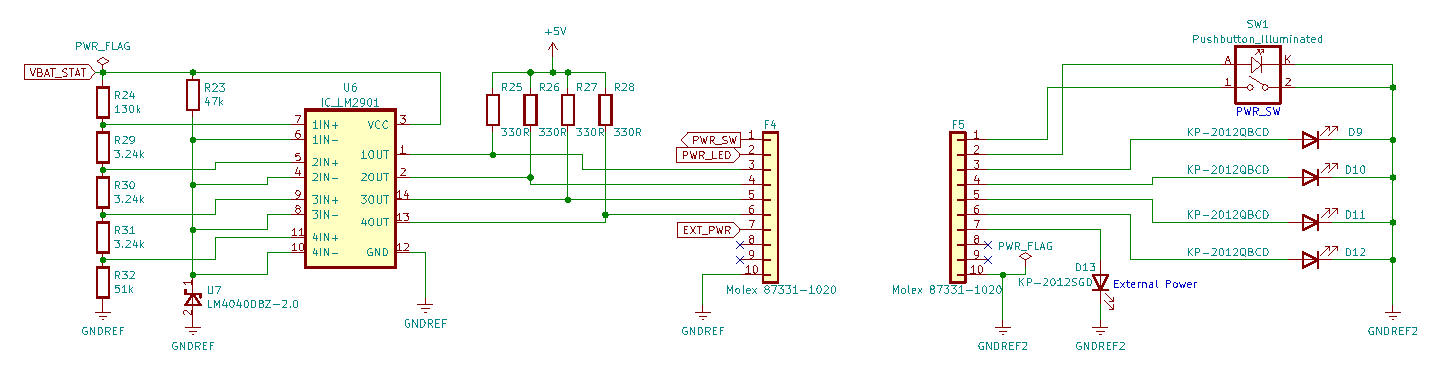
\includegraphics[width=1.0\textwidth]{Chapters/Figures/chapter3/Back_Panel.pdf}
	\caption{beRTK\textsuperscript{\textregistered} Base Station's HMI schematic diagram.}
	\label{fig:HMI_circuit}
\end{figure}

% REFERÊNCIA needed!!!!!!!!!!!!!!!!!!!!

%s--Ss--Ss--Ss--Ss--Ss--Ss--Ss--Ss--Ss--Ss--Ss--Ss--Ss--Ss--Ss--Ss--Ss--Ss--S
\subsubsection{GNSS Receiver, RTK Radio Link and Wi-Fi Transceiver}\label{sec:3232_ZEDF9P_XBEE3}

% meter aqui circuito do ZEDF9P_XBEE3
\begin{figure}[h]
	\centering
	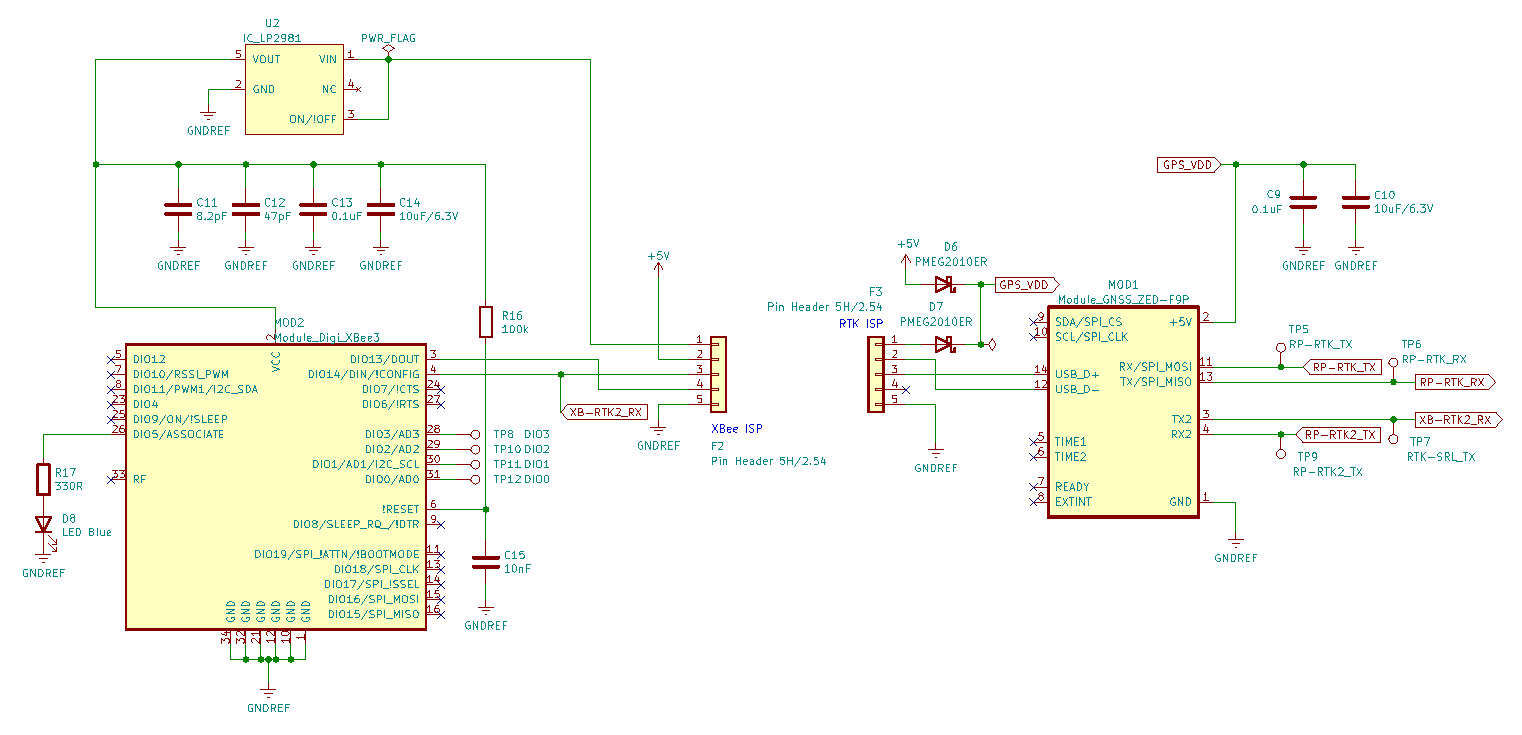
\includegraphics[width=1.0\textwidth]{Chapters/Figures/chapter3/Modules_ZEDF9P_XBEE3.pdf}
	\caption{beRTK\textsuperscript{\textregistered} Base Station's GNSS and Wi-Fi modules schematic diagram.}
	\label{fig:ZEDF9P_XBEE3_circuit}
\end{figure}

% REFERÊNCIA needed!!!!!!!!!!!!!!!!!!!!
%s--Ss--Ss--Ss--Ss--Ss--Ss--Ss--Ss--Ss--Ss--Ss--Ss--Ss--Ss--Ss--Ss--Ss--Ss--S
\subsubsection{USB Hub}\label{sec:3233_LAN9514}

% meter aqui circuito do USB_Hub_1
\begin{figure}[h]
	\centering
	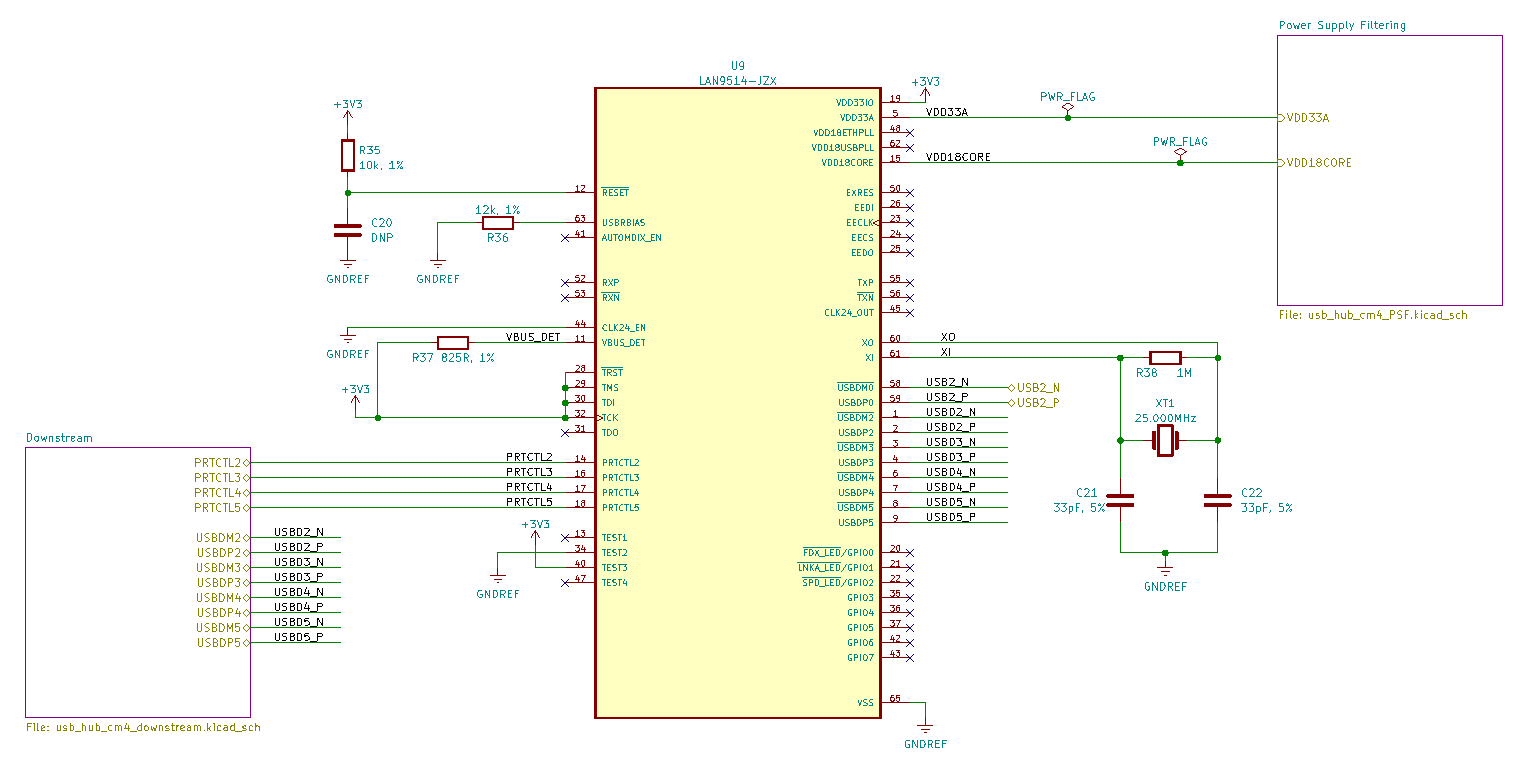
\includegraphics[width=1.0\textwidth]{Chapters/Figures/chapter3/USB_Hub_1.pdf}
	\caption{beRTK\textsuperscript{\textregistered} Base Station's USB Hub schematic diagram.}
	\label{fig:USB_Hub_1_circuit}
\end{figure}

% meter aqui circuito do USB_Hub_1
\begin{figure}[h]
	\centering
	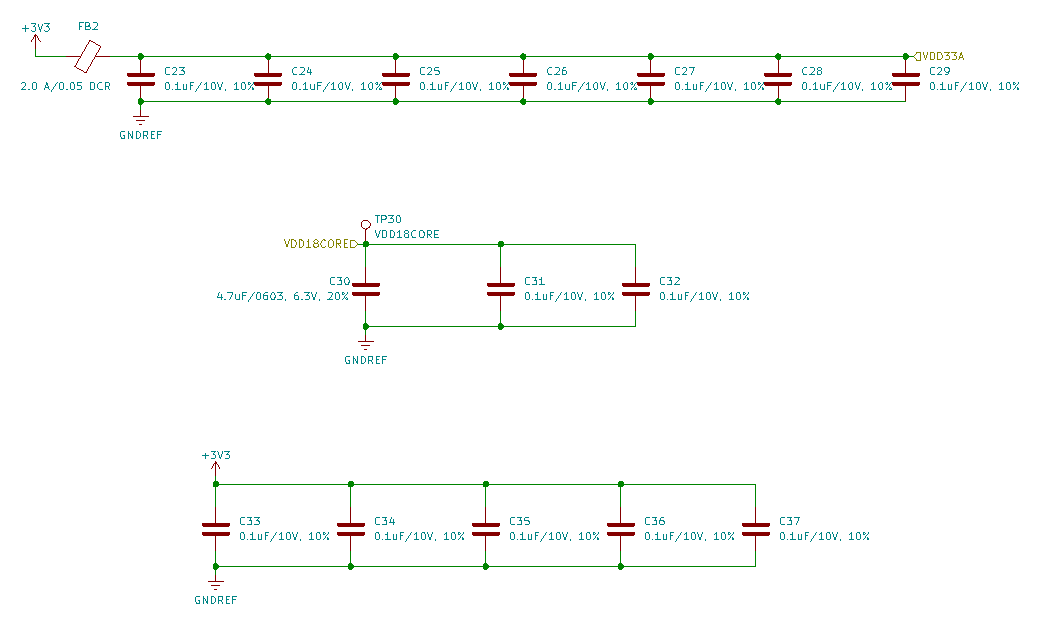
\includegraphics[width=1.0\textwidth]{Chapters/Figures/chapter3/USB_Hub_PwrSplyFiltering.pdf}
	\caption{beRTK\textsuperscript{\textregistered} Base Station's USB Hub's Power Supply Filtering schematic diagram.}
	\label{fig:USB_Hub_PwrSplyFiltering_circuit}
\end{figure}

% meter aqui circuito do USB_Hub_1
\begin{figure}[h]
	\centering
	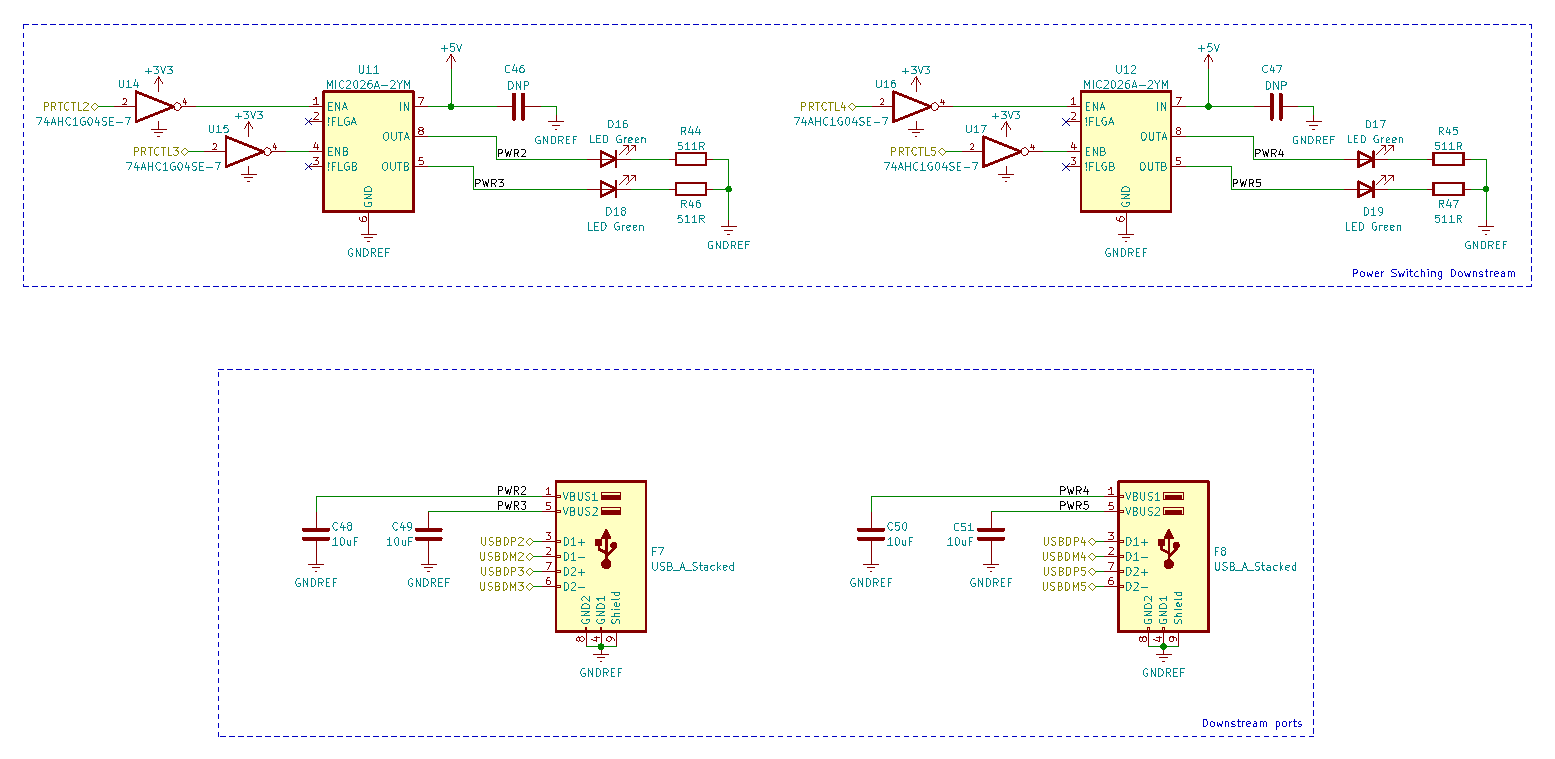
\includegraphics[width=1.0\textwidth]{Chapters/Figures/chapter3/USB_Hub_Downstream.pdf}
	\caption{beRTK\textsuperscript{\textregistered} Base Station's USB Hub's Downstream schematic diagram.}
	\label{fig:USB_Hub_Downstream_circuit}
\end{figure}

% REFERÊNCIA needed!!!!!!!!!!!!!!!!!!!!
%SSSSSSSSSSSSSSSSSSSSSSSSSSSSSSSSSSSSSSSSSSSSSSSSSSSSSSSSSSSSSSSSSSSSSSSSSSSS
\section{PCB Layout Design}\label{sec:33_PCBlayout}

